\documentclass[twoside,11pt]{starlink}
\usepackage{graphicx}
\usepackage{pdfpages}
\usepackage{float}
\usepackage[labelformat=empty]{subfig}
\usepackage[font=footnotesize]{caption}

\stardocauthors     {D.S. Berry }
\stardocdate        {12th February 2017}
\stardoctitle       {POL-2 data reduction using POL2MAP}
\stardocversion     {V1.0}
\stardocabstract    {A description and analysis of the SMURF:POL2MAP
command, including some preliminary results for a range of different
extended astronomical objects.}

\begin{document}
\scfrontmatter

\section{Introduction}
The \texttt{pol2map} command within the Starlink SMURF package creates a
vector catalogue from one or more POL2 observations.  In addition, it can
also create maps of Q, U and I --- both for individual observations and for
the co-add of all supplied observations. It accepts either raw data or
partially processed data (\emph{i.e.} Q/U/I time-streams or maps for
individual observations) as input, and will apply the required processing
to each input file to create the final catalogue.

Processing of POL2 data requires a total intensity (I) map for two reasons:

\begin{enumerate}
\item To define the level of Instrumental Polarisation (IP) expected at
each point on the sky. By default, \texttt{pol2map} evaluates and removes
this IP from
the Q and U data before creating Q and U map for each individual observation.
\item To normalise the polarised intensity values determined from the Q
and U maps to create fractional polarisation values.
\end{enumerate}

Previous methods for reducing POL2 data have usually used a total
intensity map created from one or more standard SCUBA-2 observations
(\emph{i.e.} without POL2 in the beam). However, maps created from
such observations have markedly different characteristics to maps created
from POL2 observations, due to the use of very different scanning
strategies and data reduction methods. For instance, the spatial
frequencies present in the maps are notably different, with POL2 maps
typically containing far less extended structure. Also, the Flux
Conversion Factor (FCF) used to convert power in pW into flux in Jy are
different, leading to the flux within a POL2 map being underestimated
compared to a standard SCUBA-2 map\footnote{In previous POL2 data
reduction, an attempt to correct for this difference in FCF was made
based on a fixed \emph{degradation} factor. This factor was determined
by making maps from standard SCUBA-2 observations both with and without
POL2 in the beam (but not spinning), and comparing the flux levels seen
in these maps. However, this method does not take into account any change
in FCF caused by the difference in data reduction for POL2 and non-POL2
observations, or the difference in scanning speed, and so is not
necessarily accurate.}.

To avoid these issues, the \texttt{pol2map} command uses an I map created
directly from the supplied POL2 observations themselves. It uses exactly
the same map-making procedure to create all three maps --- I, Q and U --- and
so ensures that the FCFs and spatial frequencies present in the three maps are
all consistent.

In addition, the \texttt{pol2map} command uses different filtering and
masking within the map-making process compared to previous POL2 data reduction
methods, which results in a roughly 20 \% drop in noise within the Q and U
maps and noticeably flatter backgrounds.

The extended functionality and improved results provided by
\texttt{pol2map} are bought at the cost of much greater run time. It can
take anywhere up to 3 hours per observation to run \texttt{pol2map} on a
typical SCUBA-2 capable personal computer, depending on the nature of the
observation.

\section{How to use \texttt{pol2map}}

\subsection{Getting more information about \texttt{pol2map} parameters}
As with the other Python scripts in SMURF, you can get more information
about the available parameters by doing either:

\begin{quote}
\begin{verbatim}
% pol2map --help
\end{verbatim}
\end{quote}

or

\begin{quote}
\begin{verbatim}
% smurfhelp pol2map
\end{verbatim}
\end{quote}



\subsection{Starting from raw data - extended sources\label{se1}}
This section describes how to use \texttt{pol2map} to create I, Q and U
maps, plus a vector catalogue, from the raw data files for a set of one
or more POL2 observations of an extended source.

\begin{description}
\item[Step 1]:  Create a text file listing all the raw data files for all
the observations to be included in the catalogue. Each line in the file
should contain the path to a single file, or wild-card template - the
wild-cards $*$ and $?$ are accepted. For instance:
\begin{quote}
\begin{verbatim}
% more infiles
/data/scuba2/s8?/20150716/00021/*
/data/scuba2/s8?/20150716/00023/*
/data/scuba2/s8?/20150914/00022/*
\end{verbatim}
\end{quote}

\item[Step 2]:  Run \texttt{pol2map} to create an initial I map from
the raw data files listed in your text file. The analysed intensity
values in the raw data time-streams are first converted into Q, U and I
time-streams using \texttt{smurf:calcqu} (these are stored for future use
in the directory \texttt{qudata}, specified by the \texttt{qudir}
parameter in the example command below). The \texttt{smurf:makemap} command is then used to create a
separate map from the I time-stream for each observation, using SNR-based
``auto-masking'' to define the background regions that are to be set to
zero at the end of each iteration. These maps are stored for future use
in the directory \texttt{maps}, specified by the
\texttt{mapdir} parameter in the example command below. Each map has a name of the form
\texttt{<UT\_DATE>\_<OBS\_NUM>\_<CHUNK\_NUM>\_imap.sdf}, where
\texttt{<CHUNK\_NUM>} indicates the raw data file at the start of the
contiguous chunk of data used to create the map, and is usually \texttt{0003}.
Each of these maps is compared to the specified reference map (if any)
to determine a pointing correction to be applied to the observation in
future\footnote{These pointing corrections are stored in the FITS header of
the maps created by \texttt{pol2map}.}. If no reference map is supplied, the I map created from the
first observation defines the expected source position, and is compared
with later maps to determine their pointing corrections. The reference map also
defines the output pixel grid, allowing direct pixel-by-pixel comparison between
each map created by \texttt{pol2map} and the reference map. If supplied,
the reference map should usually be a standard SCUBA-2 map of the region,
but little is lost by omitting the reference map parameter (REF).
Finally, all the individual observation I maps are co-added to form the returned
total I map, \texttt{iauto.sdf}, specified by parameter \texttt{iout}.
\begin{quote}
\begin{verbatim}
% smurf
% pol2map in=^infiles iout=iauto qout=! uout=! mapdir=maps qudir=qudata
...
...
% ls
iauto.sdf infiles maps/ pol2map.log qudata/

% ls maps
20150716_00021_0003_imap.sdf  20150716_00023_0003_imap.sdf
20150914_00022_0003_imap.sdf

% ls qudata
s8a20150716_00021_0003_IT.sdf s8a20150716_00021_0003_QT.sdf
s8a20150716_00021_0003_UT.sdf s8a20150716_00023_0003_IT.sdf
s8a20150716_00023_0003_QT.sdf s8a20150716_00023_0003_UT.sdf
s8a20150914_00022_0003_IT.sdf s8a20150914_00022_0003_QT.sdf
s8a20150914_00022_0003_UT.sdf
\end{verbatim}
\end{quote}

\item[Step 3]:  Re-run \texttt{pol2map} again, this time creating an
improved I map. The I time-streams created by the previous step, and stored
in directory \texttt{qudata}, are supplied as input instead of the raw data
files, thus avoiding the need to re-run \texttt{calcqu}. A new I map is
created from each observation, using the initial ``auto-masked'' map created
above (\texttt{iauto.sdf}) to define the background regions that are to be set
to zero at the end of each iteration. In addition, the pointing corrections
determined from the maps created in step 1 are applied during the map-making
process, resulting in better alignment of the resulting new maps. The
background estimation is done more slowly, with smaller iterative steps,
in order to achieve lower noise than the ``auto-masked'' I map - this
results in this step taking significantly longer to run than step 2. The new
I maps are placed in the same directory (\texttt{maps}) as the old I
maps, but are distinguished from them by using an upper case ``I'' in
their names (\emph{e.g.} \texttt{20150716\_00021\_0003\_Imap.sdf}). Finally,
all these individual I maps are co-added to form the improved total I map,
\texttt{iext.sdf} (the ``externally-masked'' map), specified by parameter
\texttt{iout}.

\begin{quote}
\begin{verbatim}
% pol2map in=qudata/\* iout=iext qout=! uout=! mapdir=maps mask=iauto \
          maskout1=astmask maskout2=pcamask
...
...
% ls
iauto.sdf iext.sdf infiles maps/ pol2map.log pol2map.log.1 qudata/
astmask.sdf pcamask.sdf

% ls maps
20150716_00021_0003_imap.sdf  20150716_00023_0003_imap.sdf
20150914_00022_0003_imap.sdf  20150716_00021_0003_Imap.sdf
20150716_00023_0003_Imap.sdf  20150914_00022_0003_Imap.sdf

\end{verbatim}
\end{quote}

The file \texttt{astmask.sdf} is left holding the pixel mask that defines
the region of the map that are set to zero at the end of each iteration
within \texttt{makemap}. This is an optional output and the MASKOUT1
parameter can be left unset if the mask is not required. Similarly, the
file \texttt{astmask.sdf} is left holding the pixel mask that defines the
sources regions excluded when calculating the background models (PCA, COM,
FLT) within \texttt{makemap}. These masks can come in useful when adding
in new data to a pre-existing reduction - see section~\ref{sec:addin}.

\item[Step 4]:  Re-run \texttt{pol2map} again, this time creating Q and U
maps and the final vector catalogue. This process again starts from the
time-streams created by step 1, and stored in directory \texttt{qudata}.
It uses the same auto-masked map, \texttt{iauto.sdf}, to define the
background regions that are to be set to zero at the end of each
iteration. Thus the final I, Q and U maps are all created with the same
zeroed background regions. In addition, the same slower estimate of the
background is used as in step 3, and the same pointing corrections are
also re-used. Correction for instrumental polarisation is performed,
based on the total intensity map created by step 3 (\texttt{iext.sdf}).
The Q and U maps for individual observations are placed in the same
directory (\texttt{maps}) as the I maps, and have names of the same form
as the I maps except that ``I'' is replaced by ``Q'' or ``U''. Finally,
all the individual Q and U maps are co-added to form the final Q and U
maps, \texttt{qext.sdf} and \texttt{uext.sdf}, specified by parameters
\texttt{qout} and \texttt{uout}. The three equivalent maps -
\texttt{iext.sdf}, \texttt{qext.sdf} and \texttt{uext.sdf} are then used
to create the final vector catalogue, which is placed in file
\texttt{mycat.FIT}. The vectors are de-biased to remove statistical
biasing in low SNR regions.

\begin{quote}
\begin{verbatim}
% pol2map in=qudata/\* iout=! qout=qext uout=uext mapdir=maps mask=iauto \
          ipref=iext cat=mycat debias=yes
...
...
% ls
iauto.sdf iext.sdf infiles maps/ mycat.FIT pol2map.log pol2map.log.1
pol2map.log.2 qext.sdf qudata/ uext.sdf

% ls maps
20150716_00021_0003_Imap.sdf 20150716_00021_0003_Qmap.sdf
20150716_00021_0003_Umap.sdf 20150716_00021_0003_imap.sdf
20150716_00023_0003_Imap.sdf 20150716_00023_0003_Qmap.sdf
20150716_00023_0003_Umap.sdf 20150716_00023_0003_imap.sdf
20150914_00022_0003_Imap.sdf 20150914_00022_0003_Qmap.sdf
20150914_00022_0003_Umap.sdf 20150914_00022_0003_imap.sdf

\end{verbatim}
\end{quote}


\end{description}

\subsection{Starting from pre-calculated I, Q and U time-streams}
If you have a set of pre-calculated I, Q and U time-streams for one or
more observations in a directory called \texttt{qudata}, you can use them
to create co-added  I, Q and U maps, plus a vector catalogue, by
following the procedure described in section \ref{se1} starting at step
2, but specifying the files in \texttt{qudata} as input, instead of the
raw data files:
\begin{quote}
\begin{verbatim}
% smurf
% pol2map in=qudata/\* iout=iauto qout=! uout=! mapdir=maps
\end{verbatim}
\end{quote}
Subsequent steps are as described in section \ref{se1}.


\subsection{Continuing an interrupted run of \texttt{pol2map}}
If for any reason a run of \texttt{pol2map} is interrupted, you can
continue it from where it left off, rather than starting again at the
beginning. To do this, first identify and delete any output files that were
created by the previous run of \texttt{pol2map} but which are unusable
for any reason. Output files are placed the directories specified by the
two parameters \texttt{mapdir} and \texttt{qudir}. To check if they are
usable, try accessing them in some simple way such as getting their
statistics:
\begin{quote}
\begin{verbatim}
% kappa
% stats qudata/\*
% stats maps/\*
\end{verbatim}
\end{quote}

An error will be reported by the \texttt{stats} command for any NDFs
that are corrupt (\emph{e.g.} because \texttt{makemap} or \texttt{calcqu}
terminated mid-way). Any such NDFs should be deleted.

The next step depends on the value you supply for the boolean parameter
\texttt{reuse} when re-running \texttt{pol2map}. If you accept the
default value (\texttt{yes}), then you can re-run \texttt{pol2map} with the
same list of input data files as before. In this case, the script will
identify any output files that already exist in the two output directories
and use the existing files directly rather than re-creating them from the
corresponding input files. If you set the \texttt{reuse} parameter to
\texttt{no} when re-running \texttt{pol2map}, any pre-existing output files
will be ignored and new output files will be created from the
corresponding input files using \texttt{makemap} or \texttt{qudir}.

\subsection{Adding in new observations\label{sec:addin}}
This section describes how to add data for one or more new POL2
observations into existing I, Q and U maps and vector catalogue created
by an earlier run of \texttt{pol2map}.

\begin{description}
\item[Step 1]:  Create a text file listing all the existing auto-masked I maps for
individual observations stored in the directory specified by parameter
\texttt{mapdir}, and then add in the raw data files for the new
observations. The auto-masked I maps have names that end in
"\texttt{\_imap.sdf}". For example if your raw data is stored by sub-array
in directory \texttt{sc2data}:

\begin{quote}
\begin{verbatim}
% ls maps/*imap.sdf > infiles
% echo "/sc2data/s8?/20170823/00023/*" >> infiles
\end{verbatim}
\end{quote}

\item[Step 2]:  Create a new auto-masked co-added I map including the new
observation. The \texttt{calcqu} and \texttt{makemap} commands will
be run on the new data and the resulting maps co-added with the existing
maps for the older observations to create the new map:

\begin{quote}
\begin{verbatim}
% pol2map in=^infiles iout=iauto_new qout=! uout=! mapdir=maps qudir=qudata
\end{verbatim}
\end{quote}

\item[Step 3:] You will need to decide whether to re-create all the externally
masked maps using external masks defined by the new auto-masked map. This is
the case if the auto-masked map has been changed significantly by the addition
of the new observation. To do this it is necessary to compare the old and
new mask. The old masks should have been created earlier using the
MASKOUT1 and MASKOUT2 parameters (see step 3 in section~\ref{se1}). So now
create the new masks that would be generated from the new auto-masked map.
\begin{quote}
\begin{verbatim}
% pol2map in=^infiles iout=! qout=! uout=! mapdir=maps mask=iauto_new \
          maskout1=astmask_new maskout2=pcamask_new
\end{verbatim}
\end{quote}

\item[Step 4]: Decide if the addition of the new data has changed the masks
significantly. This involves comparing \texttt{astmask.sdf} and
\texttt{astmask\_new.sdf} (and also \texttt{pcamask.sdf} and
\texttt{pcamask\_new.sdf}). One way to do this is simply to display them
side by side and then compare them by eye. For instance:
\begin{quote}
\begin{verbatim}
% gdset xw
% gdclear
% picdef mode=a xpic=2 ypic=1 prefix=a
% display astmask mode=scale low=-2 high=0 badcol=grey
% picsel a2
% display astmask_new mode=current
\end{verbatim}
\end{quote}

The source regions will be shown in white and the background regions in
grey. If they look very similar to each other, then it's probably OK to
re-use the existing externally-masked maps rather than spend hours
re-creating them using the new mask.

Another more quantitative method for comparing the masks is to compare the
number of good pixels in each:
\begin{quote}
\begin{verbatim}
% stats "'astmask,astmask_new'"
...
...
   Number of pixels used  : 230391 (61.9%)
...
...
   Number of pixels used  : 231136 (62.1%)
...
\end{verbatim}
\end{quote}

In this example, the new mask has 745 more source pixels than the old
mask. For reasons of consistency, it is desirable that the externally
masked map for each observation is created using the same mask. So if
there has been a significant change to the mask, then it is advisable
to reprocess \emph{all} observations again using the new mask.
This can potentially take a long time.

\item[Step 5]: If you decide that the mask has changed significantly and
you therefore want to reprocess all observations using the new mask,
remove the existing externally-masked maps so that they will be
re-created by the next invocation of \texttt{pol2map}. Note - this will
increase the length of time taken by step 6 enormously! Also, ensure the new
auto-masked co-add is used in place of the old one to define the masks
in future.
\begin{quote}
\begin{verbatim}
% rm mapdir/*Qmap.sdf mapdir/*Umap.sdf mapdir/*Imap.sdf
% mv iauto.sdf iauto_old.sdf
% mv iauto_new.sdf iauto.sdf
\end{verbatim}
\end{quote}

\item[Step 6]: Re-create the necessary externally masked maps and co-adds,
and then create the new vector catalogue:

\begin{quote}
\begin{verbatim}
% pol2map in=qudata/\* iout=iext_new qout=! uout=! mapdir=maps \
                       mask=iauto
% pol2map in=qudata/\* iout=! qout=qext_new uout=uext_new mapdir=maps \
                       mask=iauto ipref=iext_new cat=mycat_new debias=yes
\end{verbatim}
\end{quote}

\end{description}

\subsection{Compact sources}
If you are processing compact sources, you do not need to go through the
initial steps of creating auto-masked maps, since the mask is statically
defined as a circle of radius 30 arc-seconds. So if text file
\texttt{infiles} contains your list of raw data files, just use the
single command:

\begin{quote}
\begin{verbatim}
% pol2map in=^infiles iout=imap qout=qmap uout=umap mapdir=maps \
          mask=circle cat=mycat debias=yes
...
\end{verbatim}
\end{quote}

\subsection{Checking individual observations}
A useful way to check the visual consistency of individual observations
is to use \texttt{paste} to form a cube of the maps for all observations and
then cycle through
them in the 3D viewer in \texttt{gaia}. For instance, to check the
consistency of the auto-masked I maps, do:

\begin{quote}
\begin{verbatim}
% kappa
% ls maps/*imap.sdf > imaps
% paste in=^imaps out=icube shift=\[0,0,1\]
% gaia icube
\end{verbatim}
\end{quote}

The order of the observations within the \texttt{imaps} text file
indicates the order of the 2D slices within the cube. The same approach
can be used to check the externally masked maps (I, Q or U) by using
\texttt{Imap}, \texttt{Qmap} or \texttt{Umap} in place of \texttt{imap}
above.

If you want to remake the vector catalogue excluding one or more bad
observations, then delete all files relating to the bad observations from
both output directories (\texttt{qudir} and \texttt{mapdir}), and also
from the list of input files if you are using a list file, and then
re-run step 4 from section~\ref{se1}.

\section{A detailed description of the processing performed by \texttt{pol2map}}
To be written.

\section{IP correction}
The existing IP correction (referred to as ``PL2'') is based on the mean I, Q
and U values of Uranus observed over a range of elevations. The Q and U
values were created from POL2 observations using a method similar to
\texttt{pol2scan}. The I values were created from non-POL2 observations
using \texttt{makemap} directly. The PL2 IP model does not take the POL2
degradation factor into account - this is so that it can be applied
directly to the IP reference map supplied to pol2scan, which until now
has always been a non-POL2 map. A change has been made to
\texttt{makemap} so that when using the PL2 model, it now detects whether
the IP reference map was created from POL2 data, and if so, multiplies it
by the canonical POL2 degradation factor at 850 $\mu m$ (1.35).

In addition, an entirely new IP model called ``PL3'' has been created
from the same set of Uranus observations. The Q, U and I maps were all
made from POL2 data using a circular mask of 30 arc-seconds radius and a
\texttt{makemap} configuration similar to that used by \texttt{pol2map}
in ``external mask'' mode. It was necessary to remove the COM model, as
including the COM model made the scatter of Q and U values about the fit
much larger.

The plots in this section compares the measured and fitted values for the
basic parameters of PL2 and PL3. Figures~\ref{fig:ip1} and~\ref{fig:ip2}
show that the overall level of instrumental polarisation is higher in PL3
than in PL2. This is because PL3 takes account of the POL2 degradation
when forming the fractional polarisation (by virtue of the fact that the
I values are derived from POL2 data), whereas PL2 does not. By default,
\texttt{makemap} now uses the PL3 model if the IP reference map was
created from POL2 data, and the PL2 model otherwise.

It is disappointing that the scatter of the measured values around the
fit are if anything worse in PL3 than in PL2, given the significant
reduction in the noise visible in the maps created using \texttt{pol2map}
and presented in section~\ref{sec:results}.

\begin{figure}
\centering
\begin{minipage}{.45\textwidth}
  \centering
  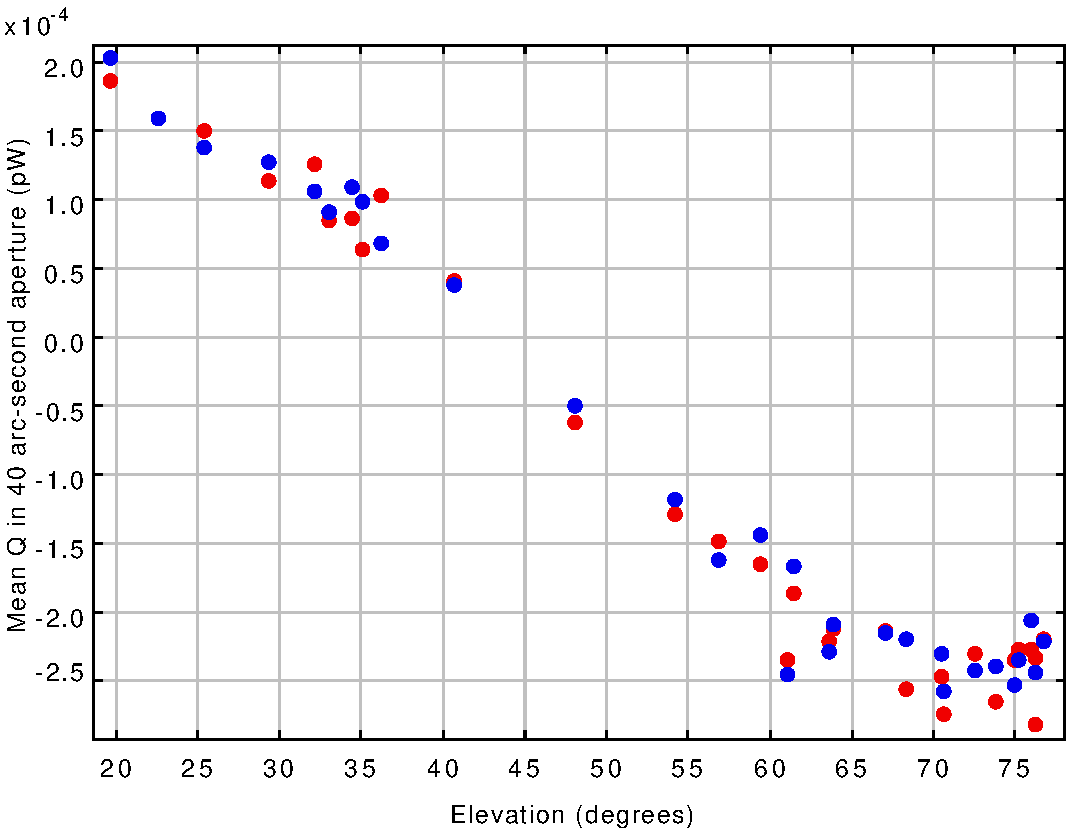
\includegraphics[width=.95\linewidth]{ip/fig1}
  \captionof{figure}{The measured mean Q values in PL2 (red) and PL3 (blue)}
\end{minipage}
~~
\begin{minipage}{.45\textwidth}
  \centering
  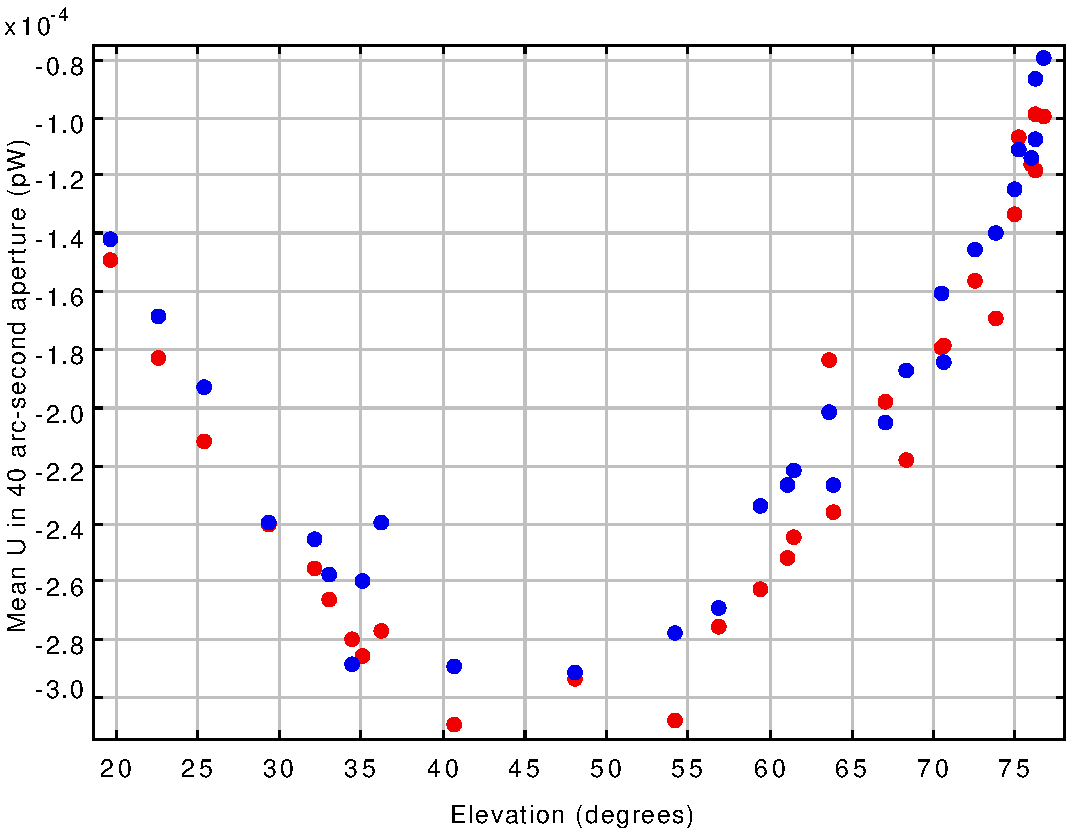
\includegraphics[width=.95\linewidth]{ip/fig2}
  \captionof{figure}{The measured mean U values in PL2 (red) and PL3 (blue)}
\end{minipage}
\end{figure}


\begin{figure}
\centering
\begin{minipage}{.45\textwidth}
  \centering
  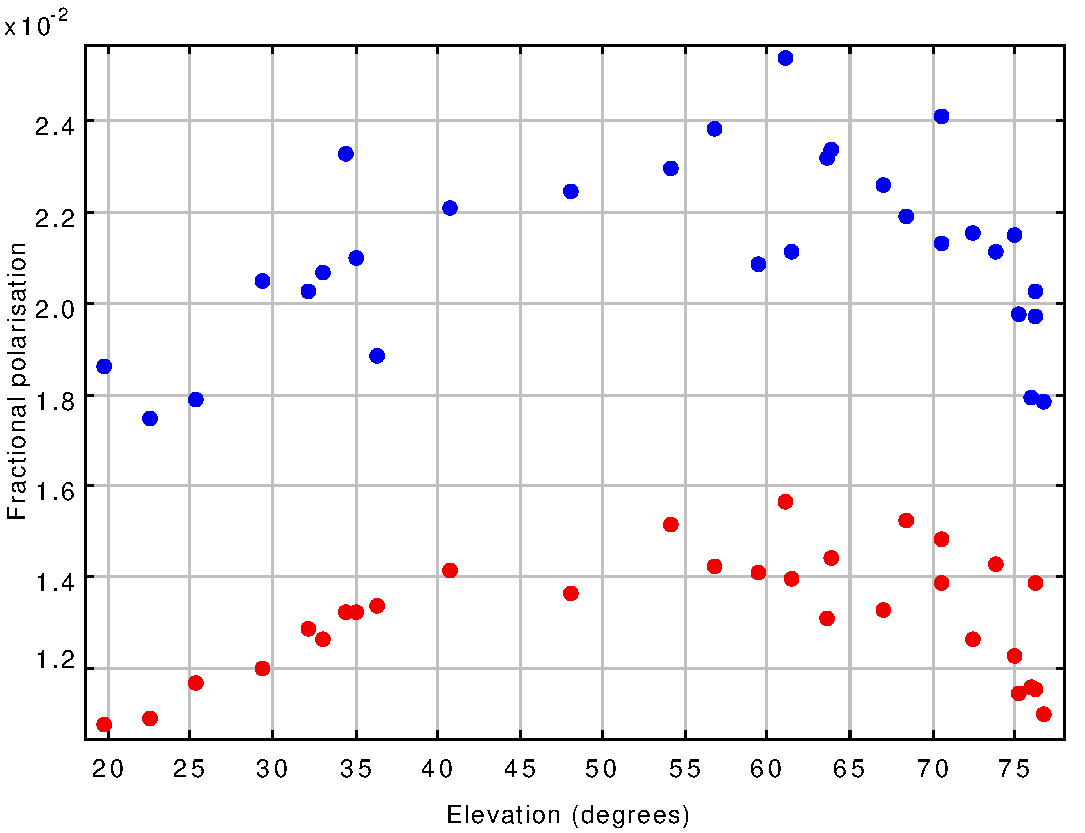
\includegraphics[width=.95\linewidth]{ip/fig3}
  \captionof{figure}{The measured fractional polarisation values in PL2 (red) and PL3 (blue)}
  \label{fig:ip1}
\end{minipage}
~~
\begin{minipage}{.45\textwidth}
  \centering
  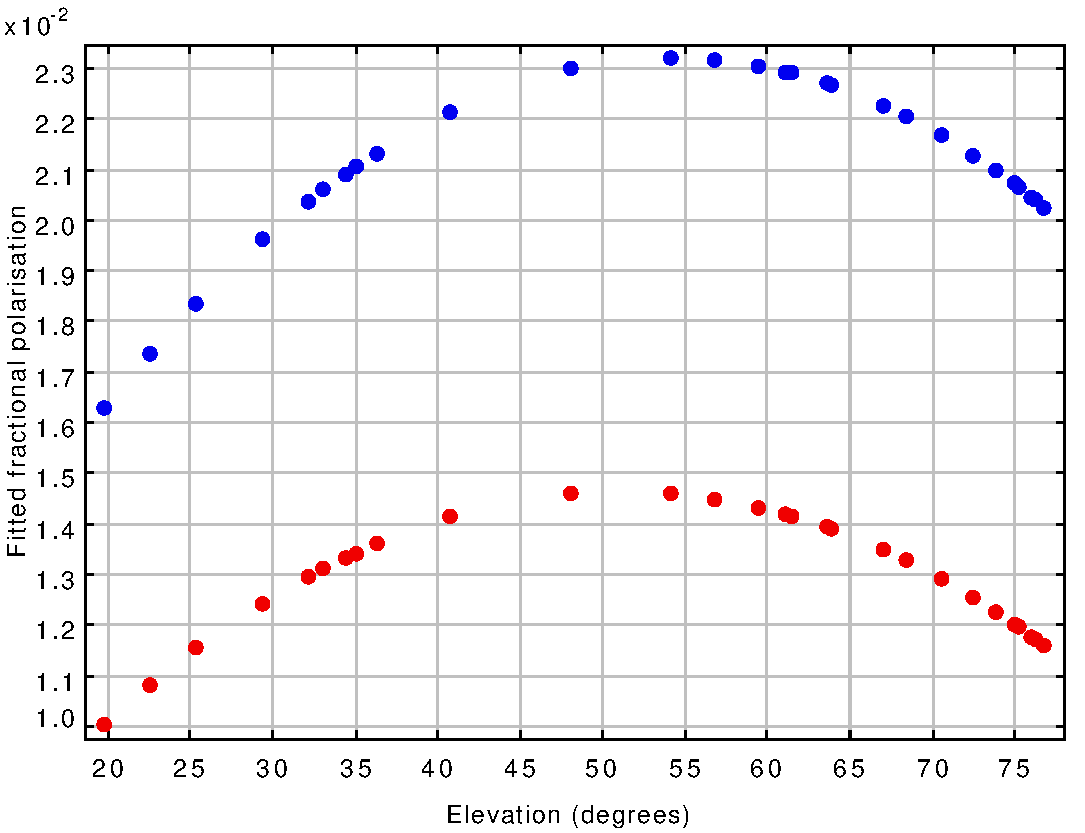
\includegraphics[width=.95\linewidth]{ip/fig4}
  \captionof{figure}{The fitted  fractional polarisation values in PL2 (red) and PL3 (blue)}
  \label{fig:ip2}
\end{minipage}
\end{figure}


\begin{figure}
\centering
\begin{minipage}{.45\textwidth}
  \centering
  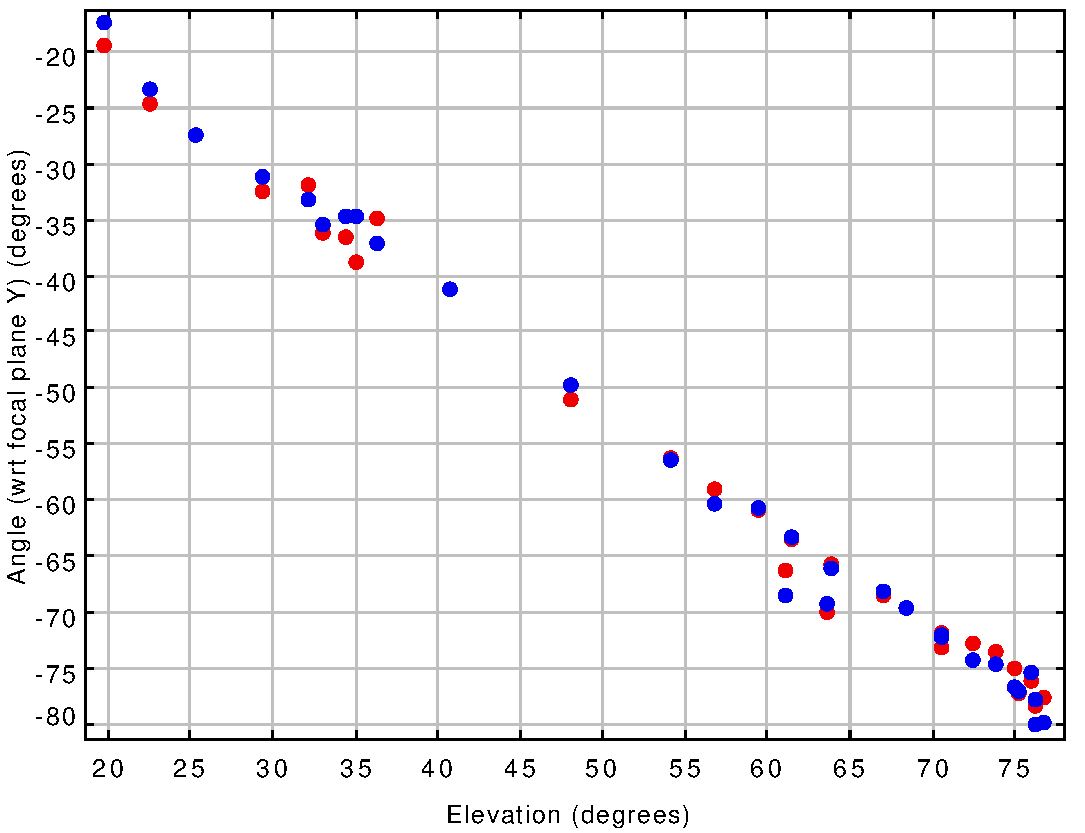
\includegraphics[width=.95\linewidth]{ip/fig5}
  \captionof{figure}{The measured polarisation angles in PL2 (red) and
                     PL3 (blue), with respect to the focal plane Y axis.}
\end{minipage}
~~
\begin{minipage}{.45\textwidth}
~~
  \centering
\end{minipage}
\end{figure}


\section{Example results from \texttt{pol2map} compared to \texttt{pol2scan}\label{sec:results}}
This section presents some very preliminary results produced by
\texttt{pol2map} for a range of different extended astronomical objects,
and compares these with equivalent results produced using the old
\texttt{pol2scan} script.

Note, these results have not been verified completely - there may be
serious issues present that need addressing within the software. These
reductions should be repeated by other people, and some independent
verification and analysis performed.

The same automatically generated plots are shown for each object:
\begin{enumerate}
\item Q and U maps: \texttt{pol2scan} maps followed by \texttt{pol2map}
maps with and without IP correction.
\item Q and U Signal-to-Noise maps: \texttt{pol2scan} maps followed by
\texttt{pol2map} maps with and without IP correction.
\item Q/U pixel errors (central region only): scatter plots compare
\texttt{pol2scan} error values compared to \texttt{pol2map}.
\item I map errors compared to Q/U map errors: all from \texttt{pol2map}
\item pol2map I map compared to non-POL2 SCUBA-2 map: two display scales
are used to highlight the bright regions and the faint regions for
comparison. The non-POL2 maps are corrected using the canonical
degradation factor (1.35 at 850 $\mu m$) before being displayed. A
difference map is included - ideally this would be a smooth map
containing just the extra extended structure present in the non-POL2 maps
but not present in the POL2 maps. In fact the presence of small scale
structures suggest he degradation factor of 1.35 may not always be
appropriate.
\item Polarised intensity maps: these are binned 3x3 to produce 12
arc-second pixels. The de-biased maps contain many bad pixels (shown in
grey) where the polarised intensity is less than the noise.
\item Polarised intensity Signal-to-Noise maps: also binned to create 12
arc-second pixels.
\item De-biased vector maps - binned 5x5 and cut at $(dp<3)\&\&(dang<10)$
\end{enumerate}

The red contours shown in some images indicate the areas that were used
to create the associated statistics or plots shown on the same page. All
maps shown on a single page share the same display scale, unless
otherwise noted.

Points to note:
\begin{enumerate}
\item The time taken to process a set of observations using
\texttt{pol2map} can be five times more than using \texttt{pol2scan}.
\item The backgrounds in the Q and U produced by \texttt{pol2map} are much
flatter and have around $30\%$ less noise than the equivalent maps
produced by \texttt{pol2scan}.
\item The on-source SNR values are higher for \texttt{pol2map} than for
\texttt{pol2scan}.
\item The errors in the I pixel values created from POL2 data are similar
in magnitude to the Q and U errors created from the same data. This means
that performing IP correction with these I maps will not add
significantly  to the noise in the final maps.
\item The I maps created from POL2 data have flatter backgrounds than
those created from non-POL2 data.
\item The I maps created from POL2 data have a higher NEFD than those
created from non-POL2 data.
\end{enumerate}



\subsection{Serpens - field 1}
These maps are made from 21 observations of Serpens field 1 taken
between 20160420 and 20160522.

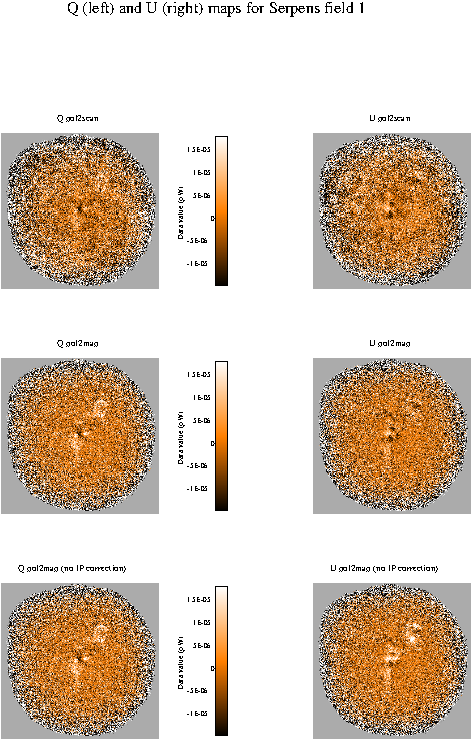
\includepdf[pages={-}]{figs/fig2.pdf}
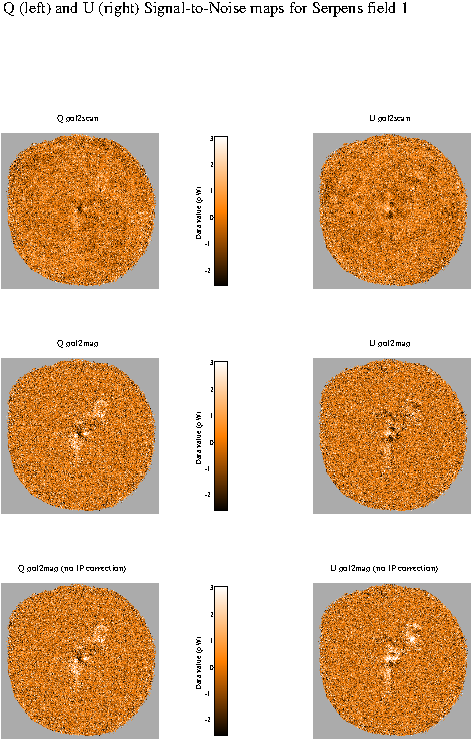
\includepdf[pages={-}]{figs/fig3.pdf}
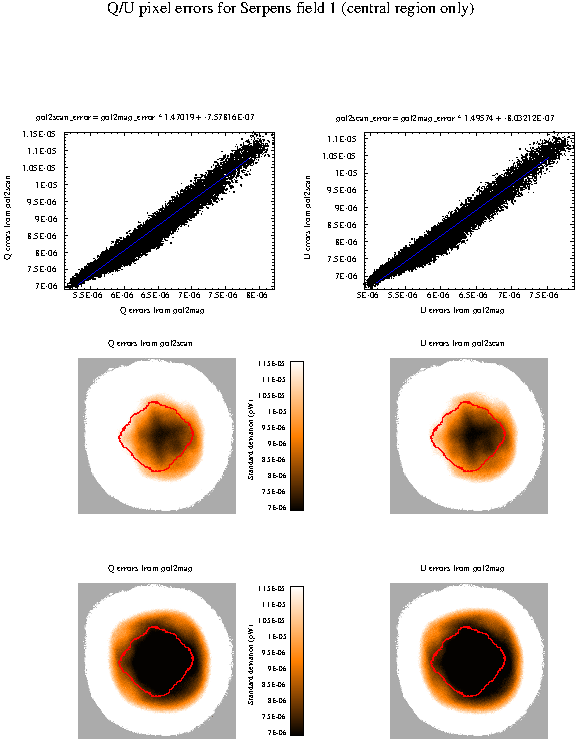
\includepdf[pages={-}]{figs/fig4.pdf}
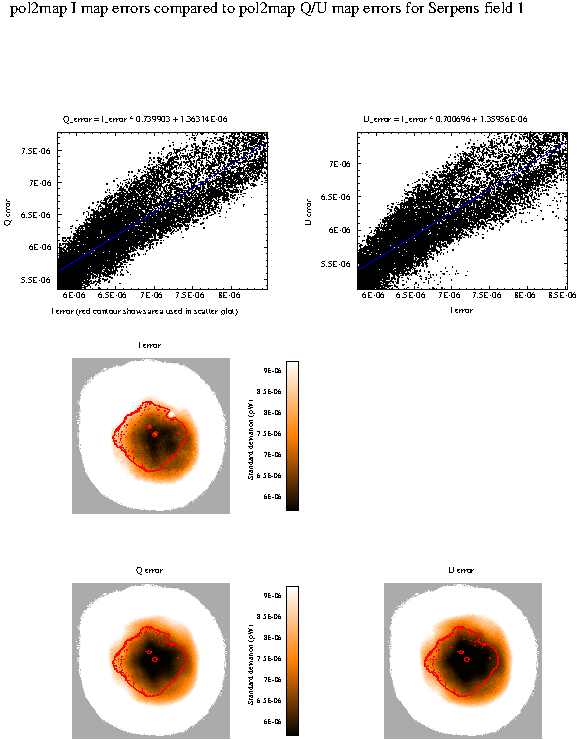
\includepdf[pages={-}]{figs/fig5.pdf}
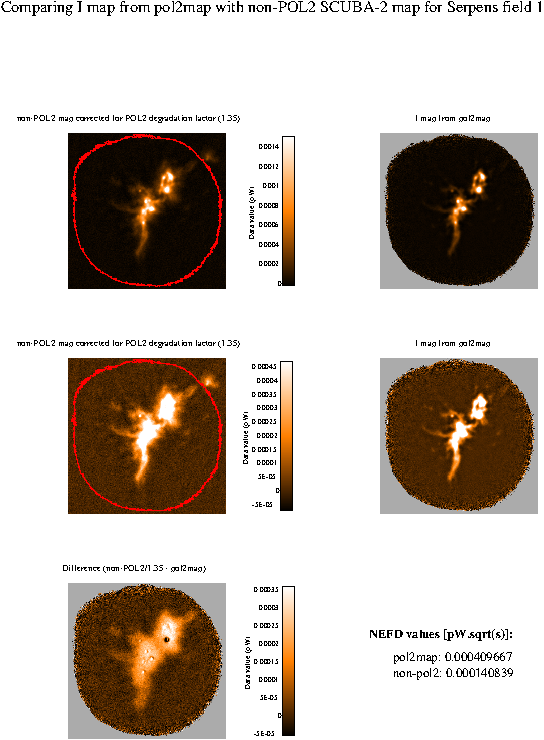
\includepdf[pages={-}]{figs/fig6.pdf}
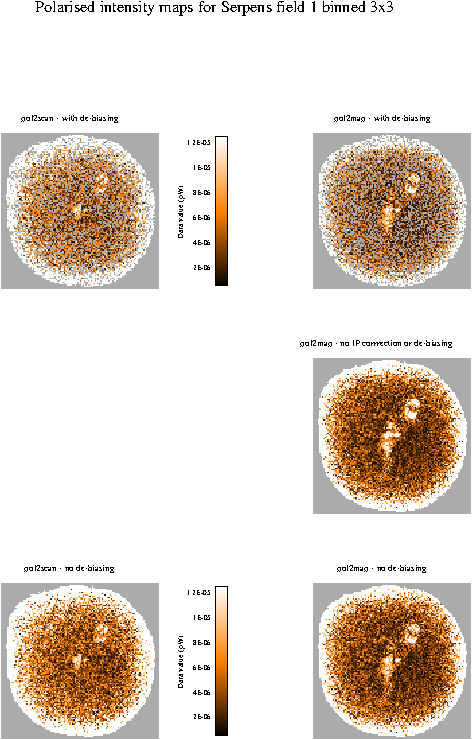
\includepdf[pages={-}]{figs/fig7.pdf}
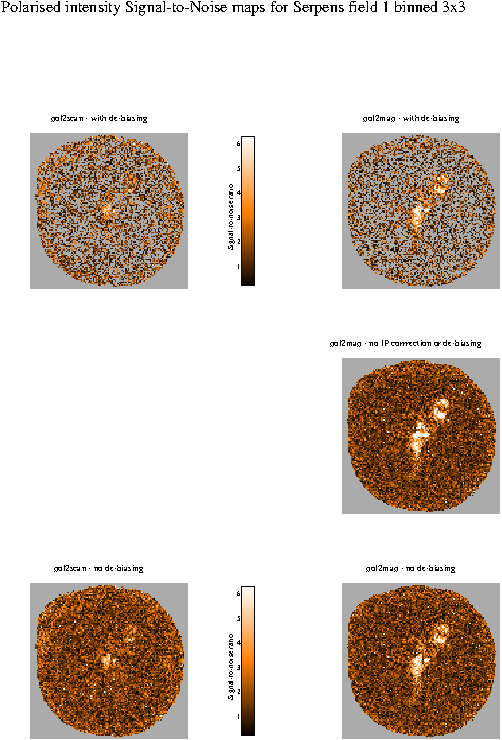
\includepdf[pages={-}]{figs/fig8.pdf}
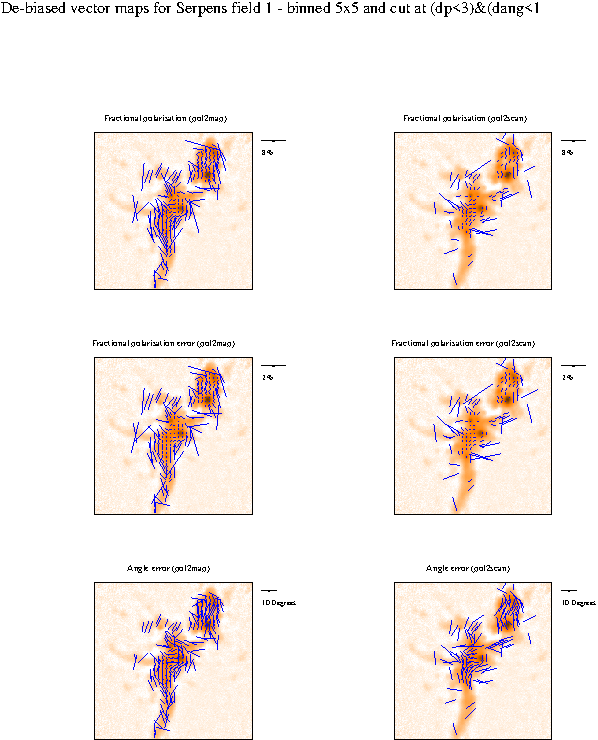
\includepdf[pages={-}]{figs/fig9.pdf}

\subsection{G34}
These maps are made from 4 observations of G34 taken on 20160729.

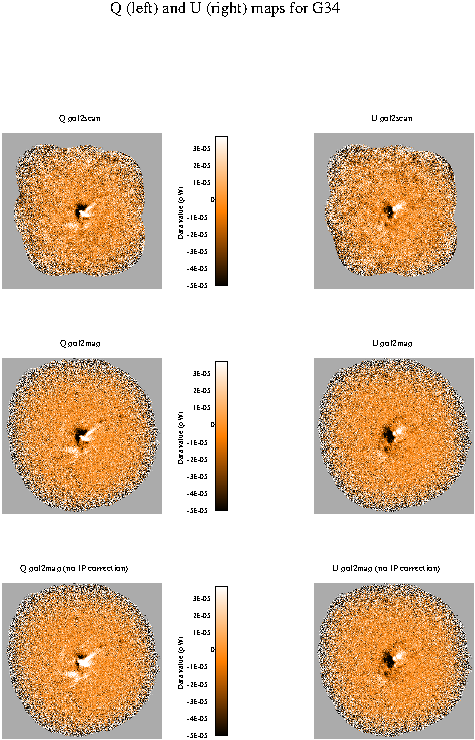
\includepdf[pages={-}]{figs/fig11.pdf}
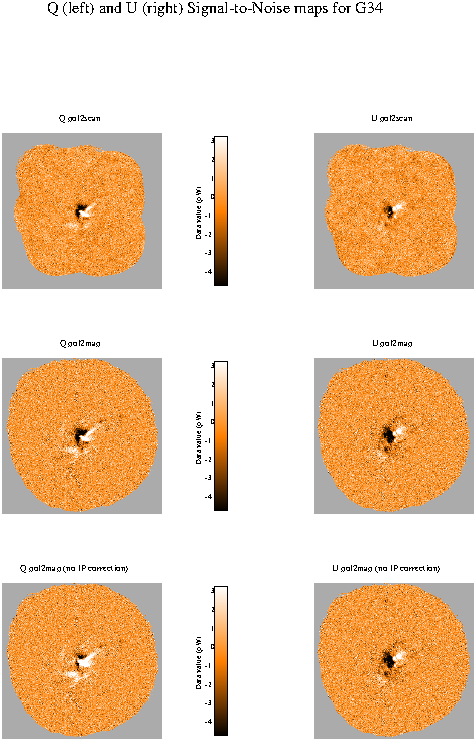
\includepdf[pages={-}]{figs/fig12.pdf}
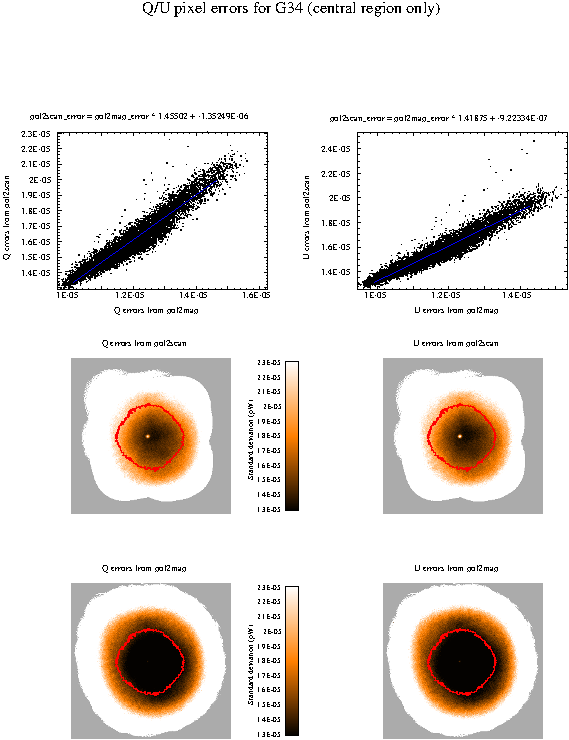
\includepdf[pages={-}]{figs/fig13.pdf}
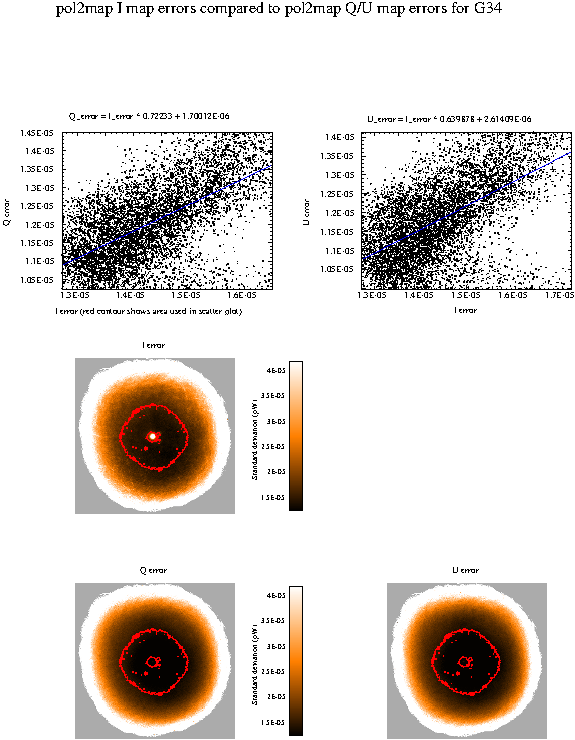
\includepdf[pages={-}]{figs/fig14.pdf}
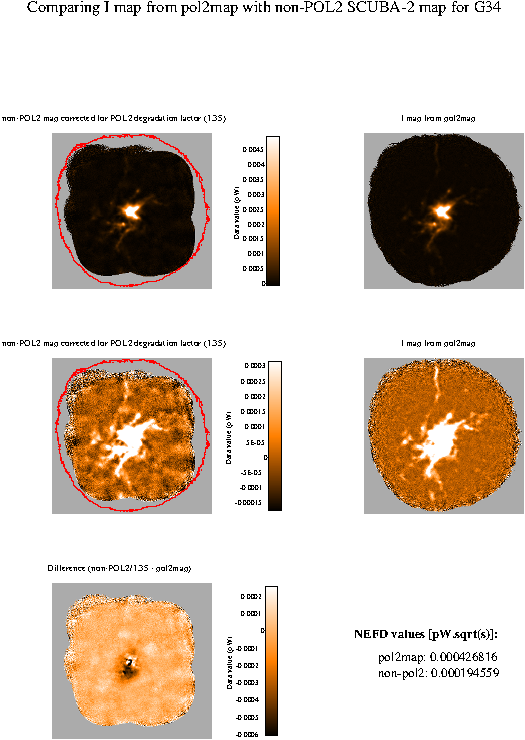
\includepdf[pages={-}]{figs/fig15.pdf}
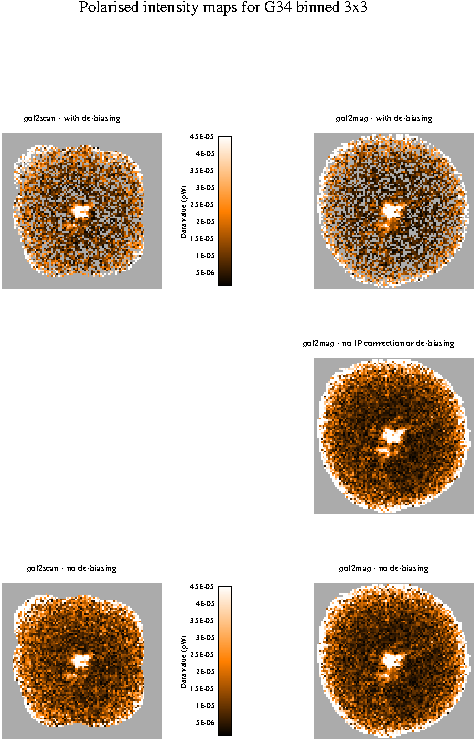
\includepdf[pages={-}]{figs/fig16.pdf}
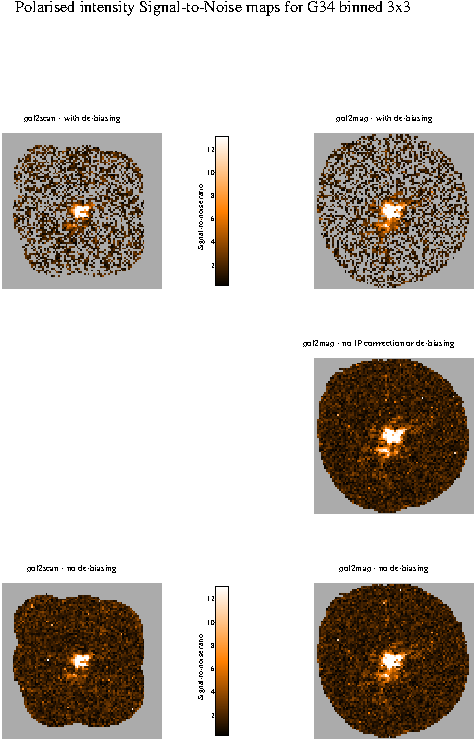
\includepdf[pages={-}]{figs/fig17.pdf}
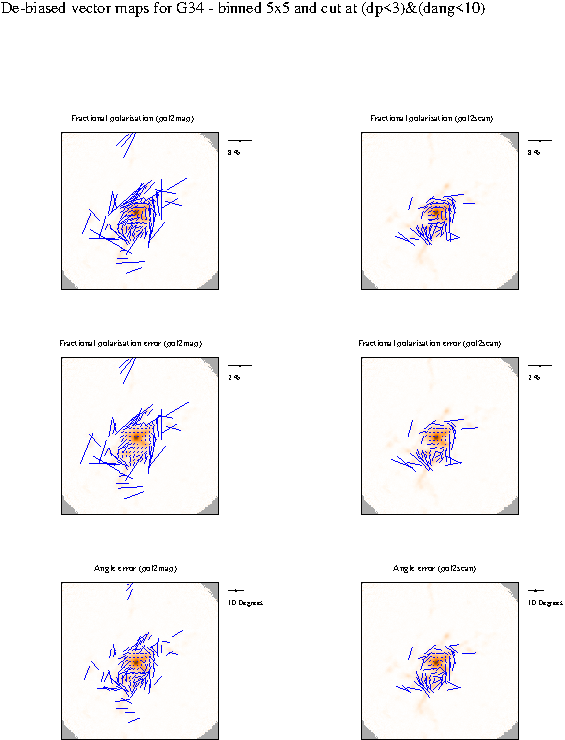
\includepdf[pages={-}]{figs/fig18.pdf}

\subsection{IC 5146}
These maps are made from 19 observations of IC 5146 taken between
20160523 and 20160910.

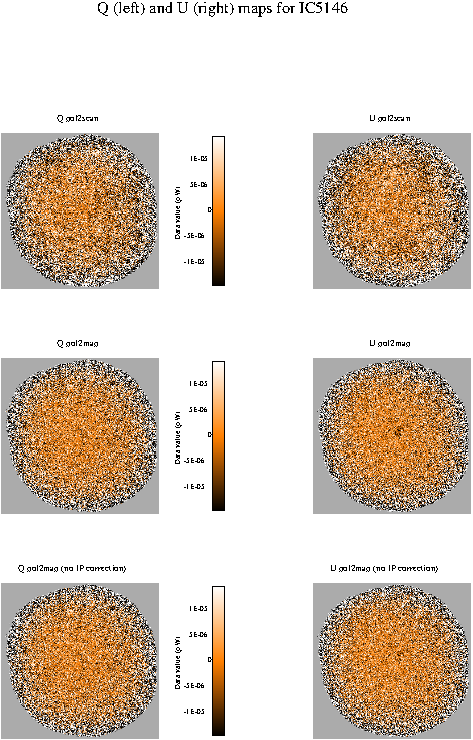
\includepdf[pages={-}]{figs/fig20.pdf}
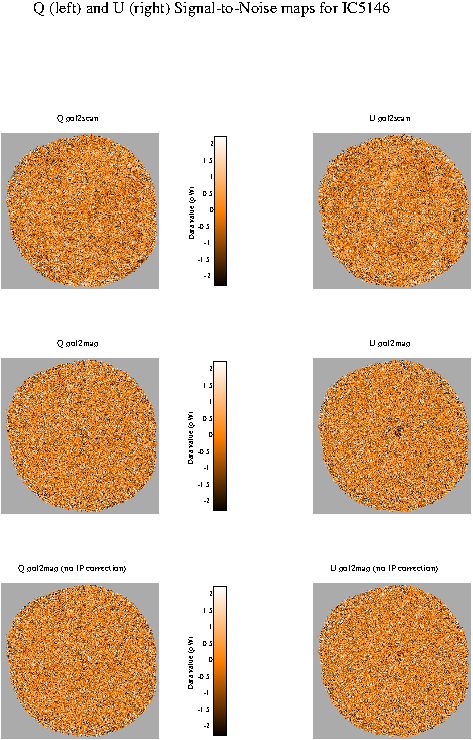
\includepdf[pages={-}]{figs/fig21.pdf}
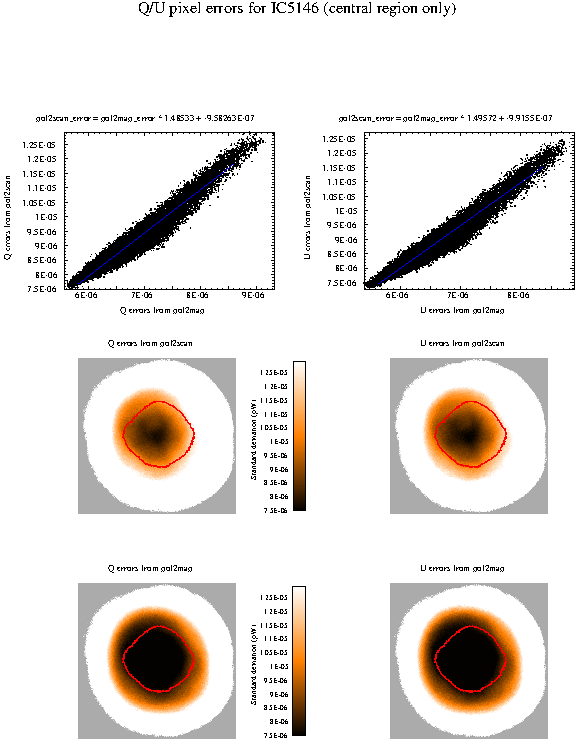
\includepdf[pages={-}]{figs/fig22.pdf}
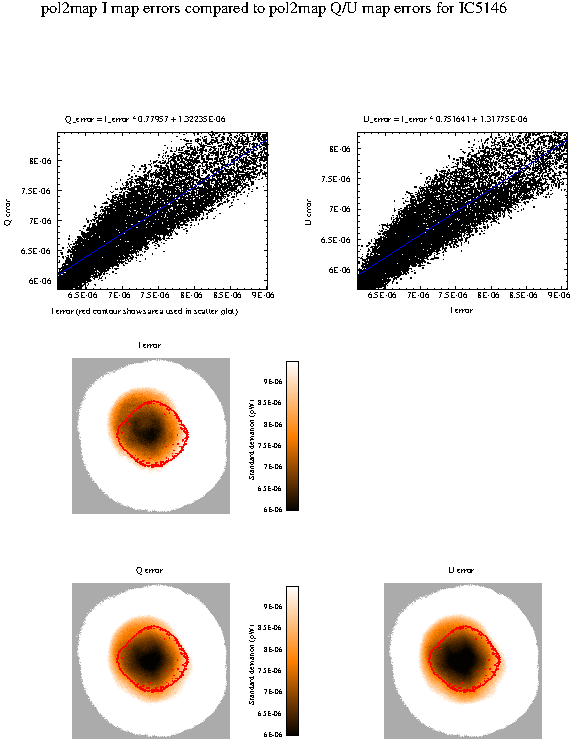
\includepdf[pages={-}]{figs/fig23.pdf}
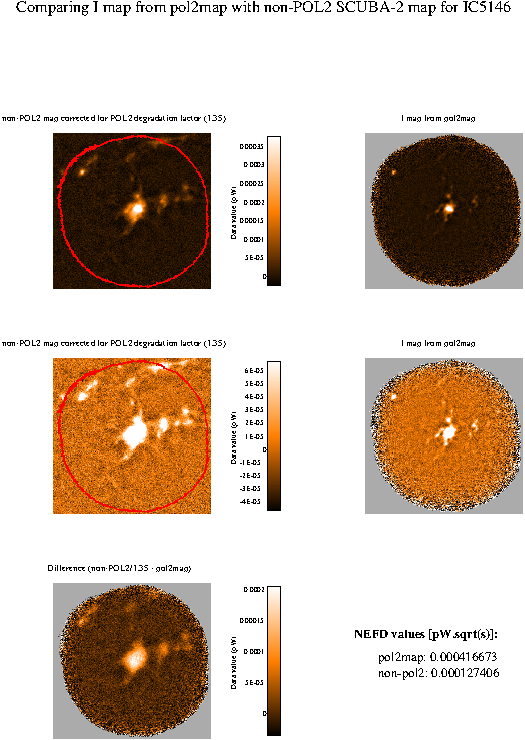
\includepdf[pages={-}]{figs/fig24.pdf}
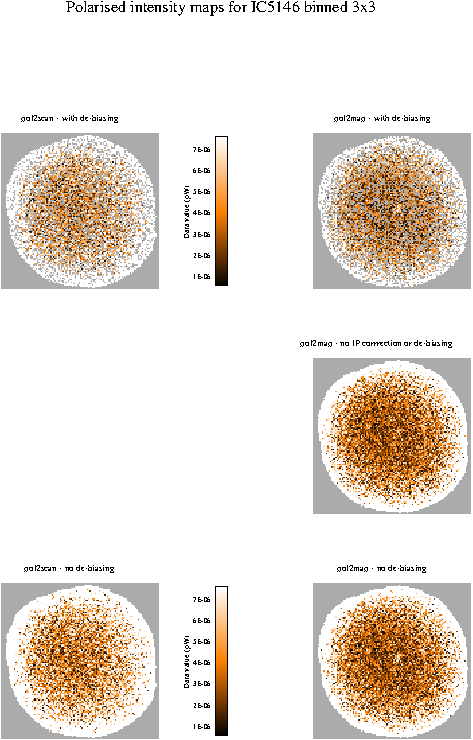
\includepdf[pages={-}]{figs/fig25.pdf}
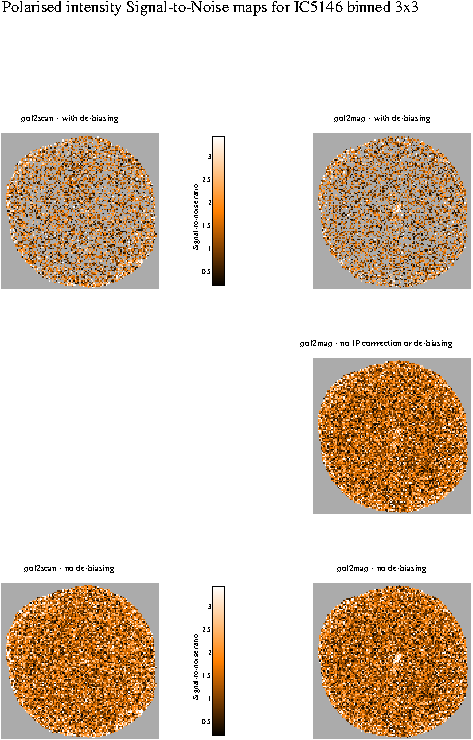
\includepdf[pages={-}]{figs/fig26.pdf}
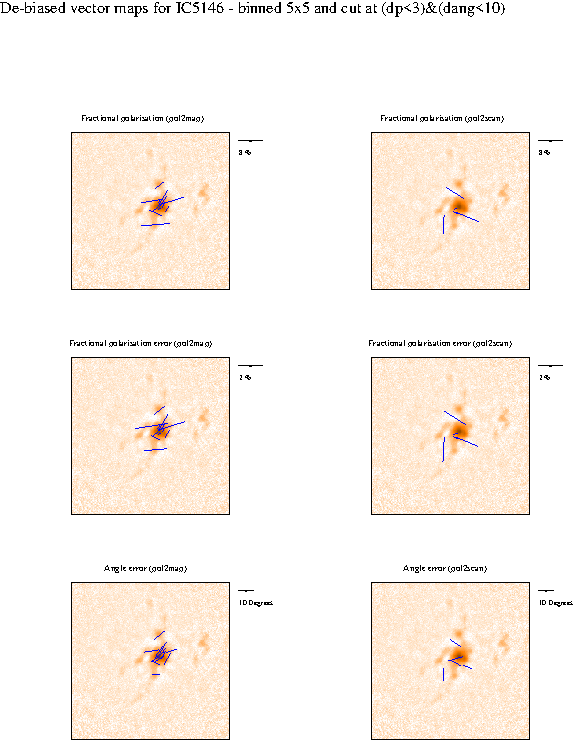
\includepdf[pages={-}]{figs/fig27.pdf}


\subsection{DR 21}
These maps are made from 13 observations of DR 21 taken between 20150716 and
20150918.

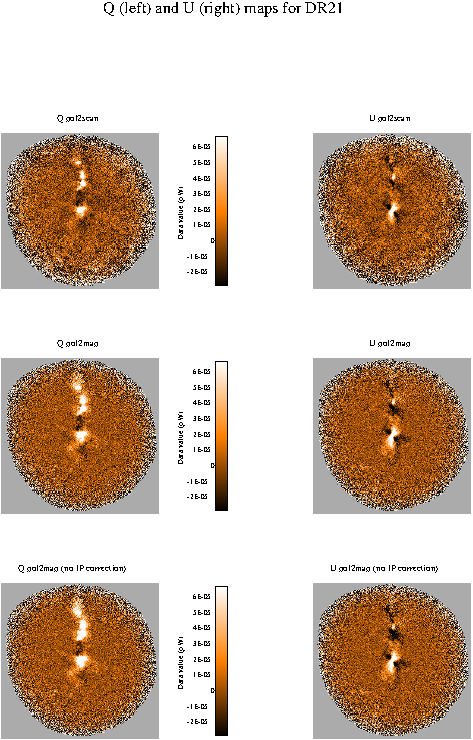
\includepdf[pages={-}]{figs/fig29.pdf}
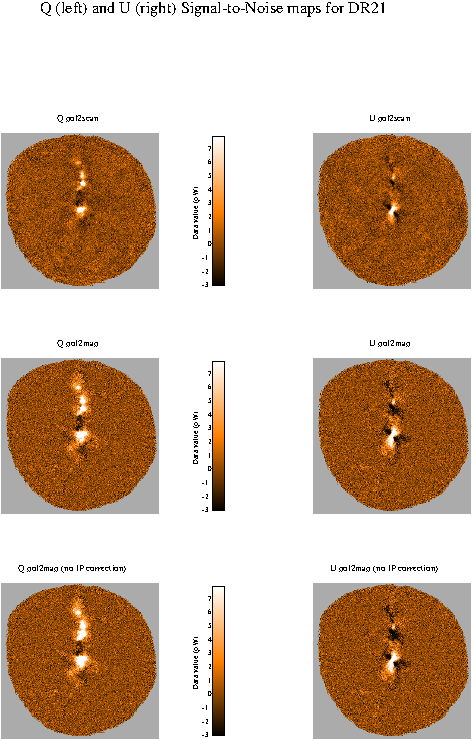
\includepdf[pages={-}]{figs/fig30.pdf}
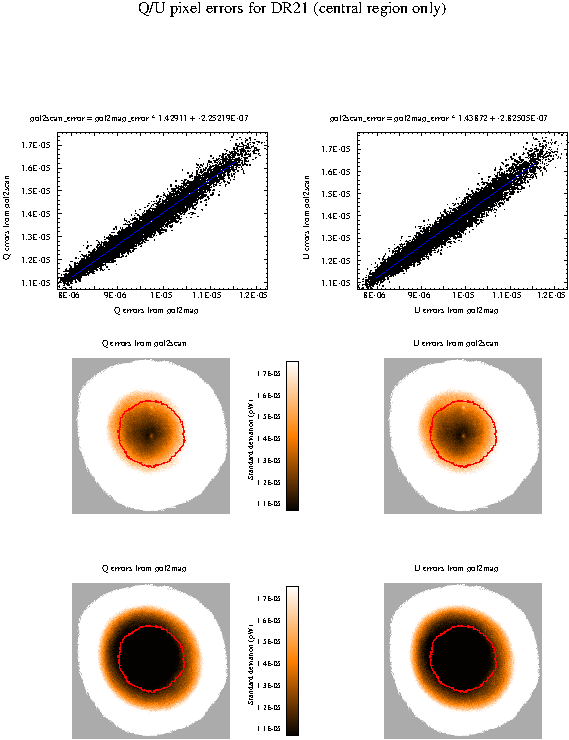
\includepdf[pages={-}]{figs/fig31.pdf}
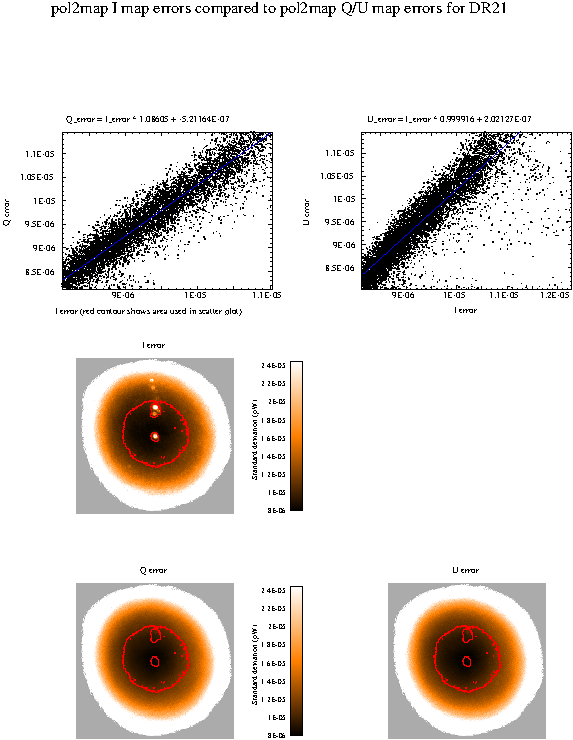
\includepdf[pages={-}]{figs/fig32.pdf}
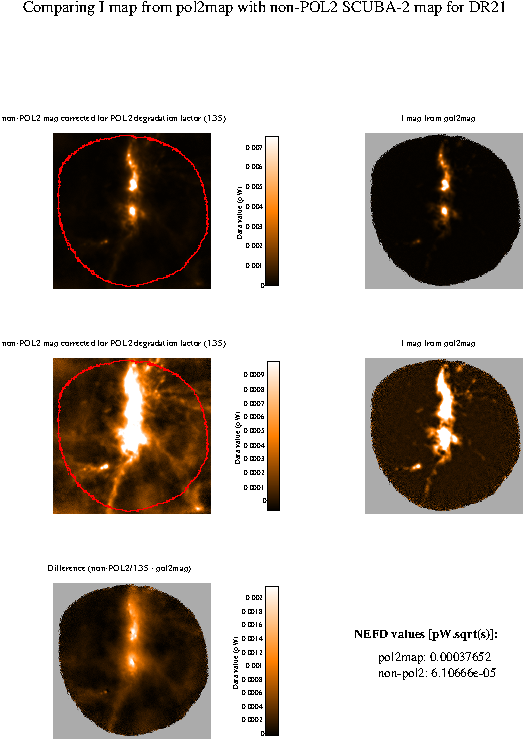
\includepdf[pages={-}]{figs/fig33.pdf}
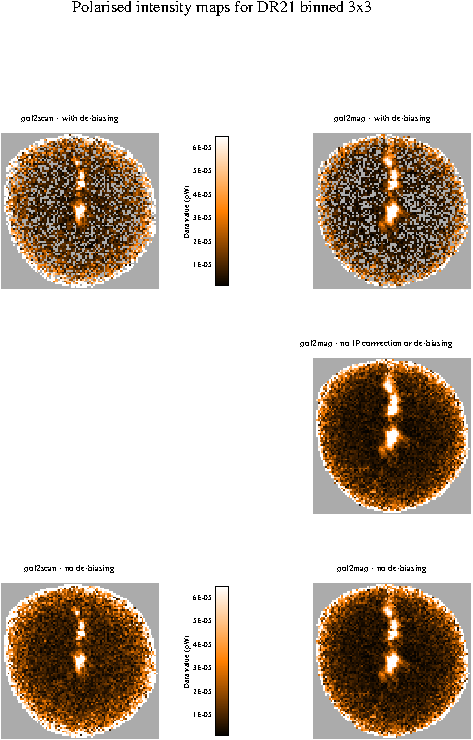
\includepdf[pages={-}]{figs/fig34.pdf}
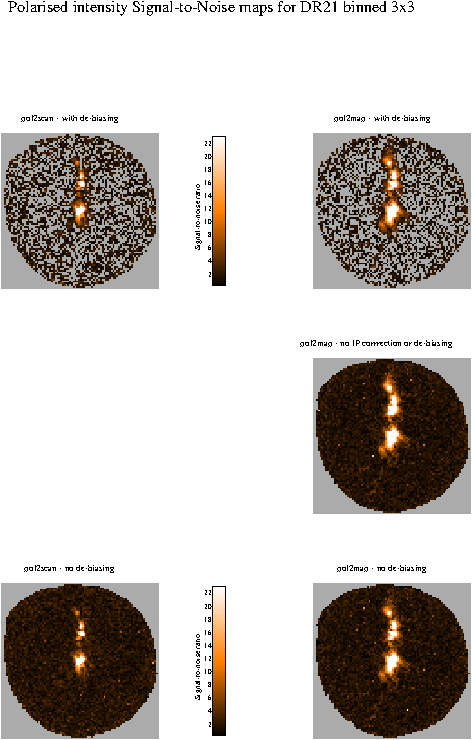
\includepdf[pages={-}]{figs/fig35.pdf}
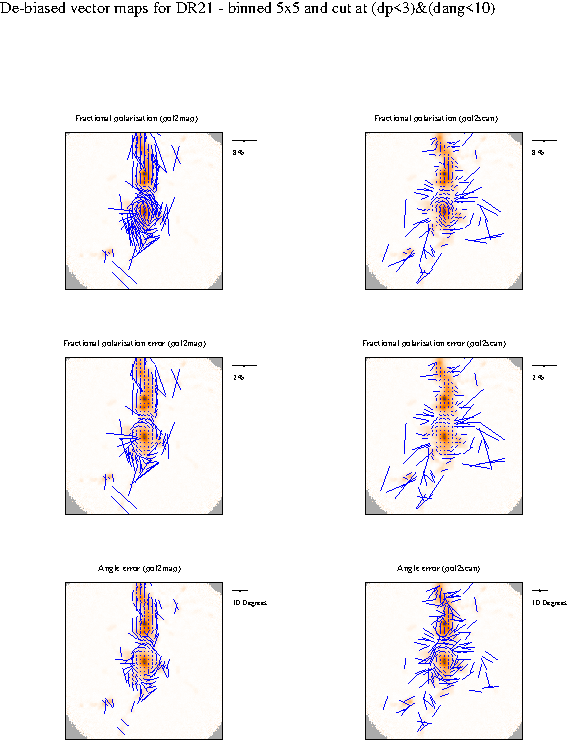
\includepdf[pages={-}]{figs/fig36.pdf}


\subsection{Perseus b1}
These maps are made from 8 observations of Perseus b1 taken between
20160908 and 20160911.

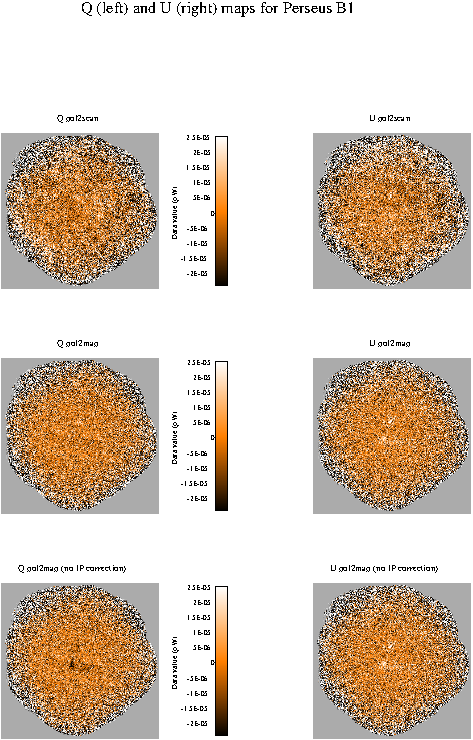
\includepdf[pages={-}]{figs/fig38.pdf}
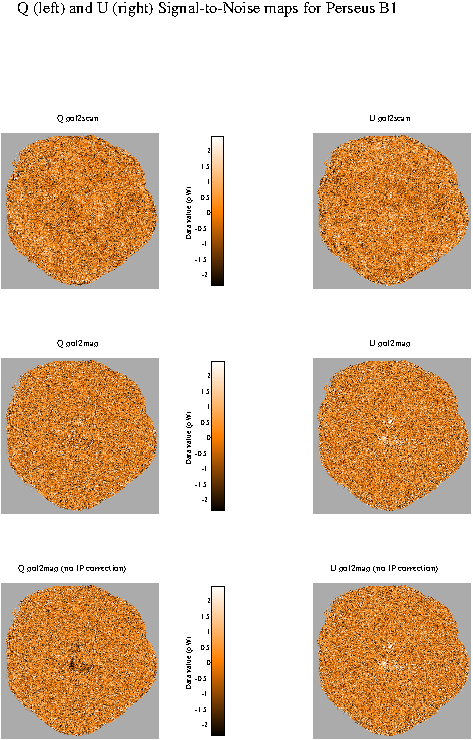
\includepdf[pages={-}]{figs/fig39.pdf}
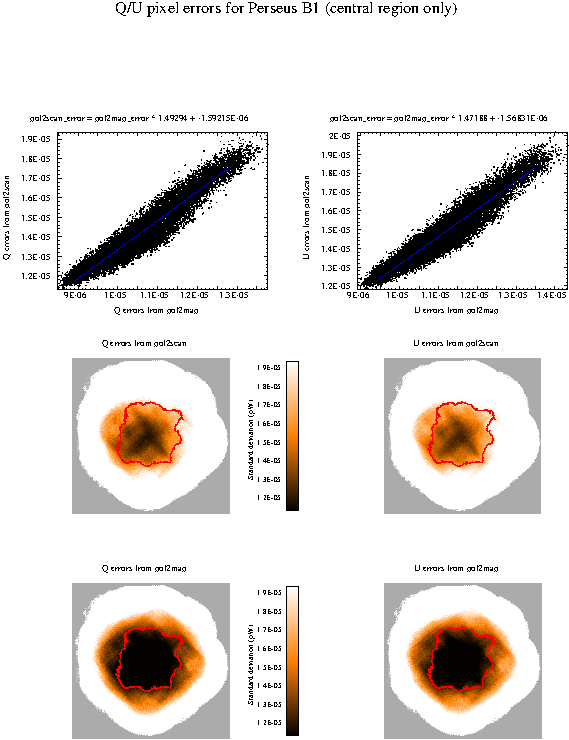
\includepdf[pages={-}]{figs/fig40.pdf}
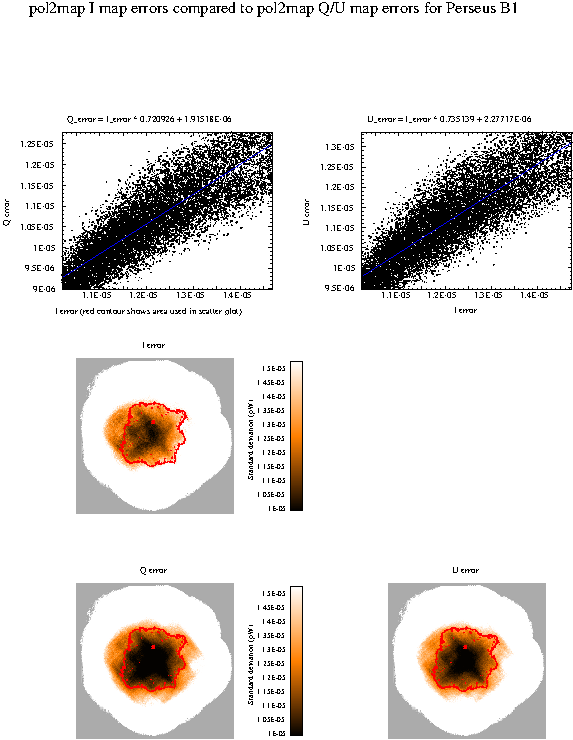
\includepdf[pages={-}]{figs/fig41.pdf}
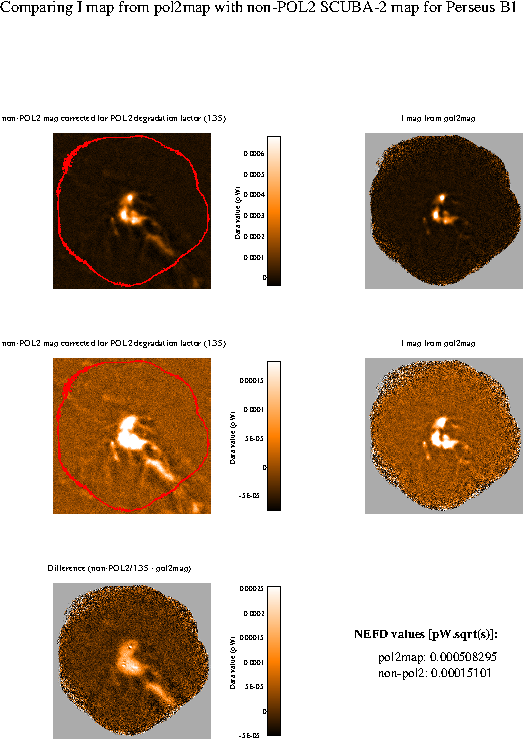
\includepdf[pages={-}]{figs/fig42.pdf}
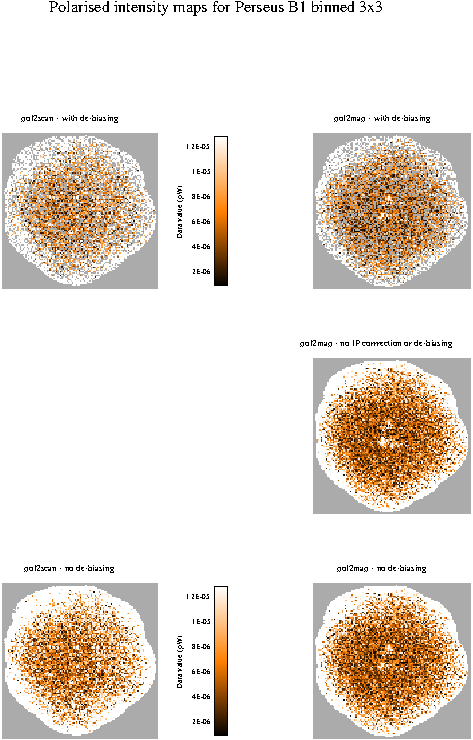
\includepdf[pages={-}]{figs/fig43.pdf}
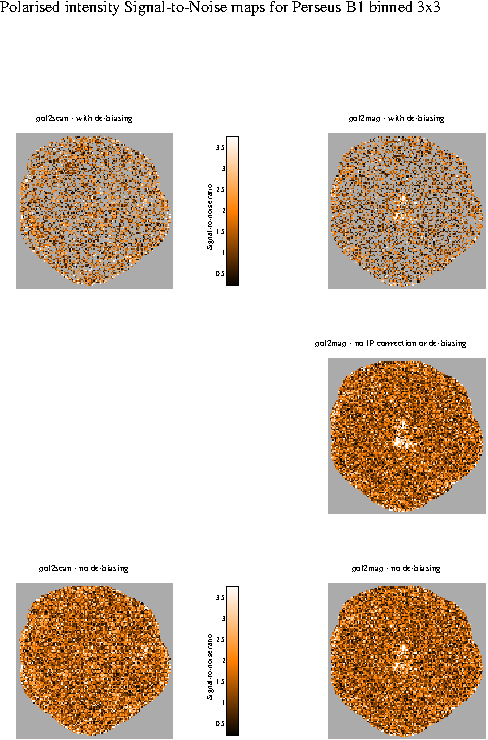
\includepdf[pages={-}]{figs/fig44.pdf}
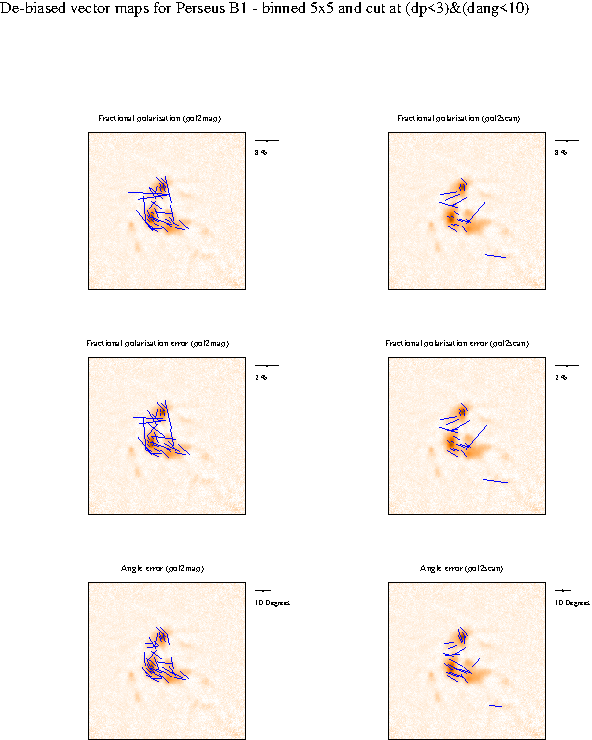
\includepdf[pages={-}]{figs/fig45.pdf}

\subsection{Ophiuchus - field 3}
These maps are made from 18 observations of Ophiuchus field 3 taken between
20160522 and 20160910.

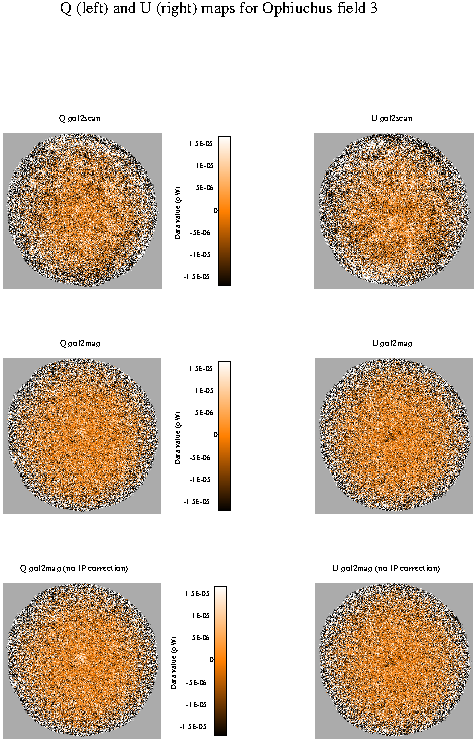
\includepdf[pages={-}]{figs/fig47.pdf}
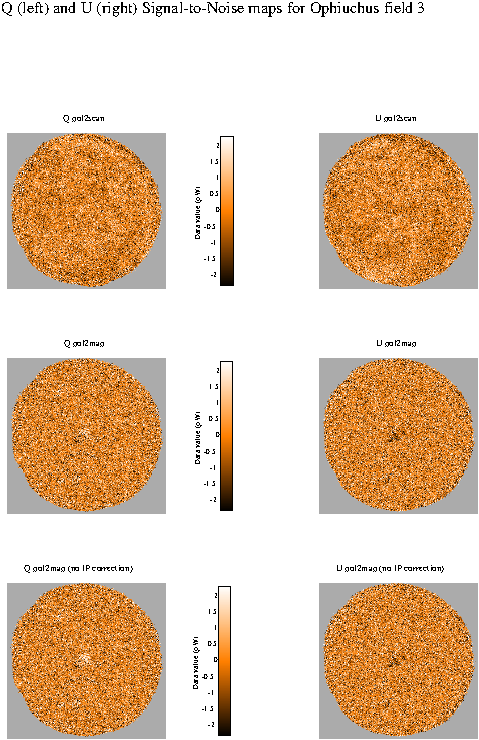
\includepdf[pages={-}]{figs/fig48.pdf}
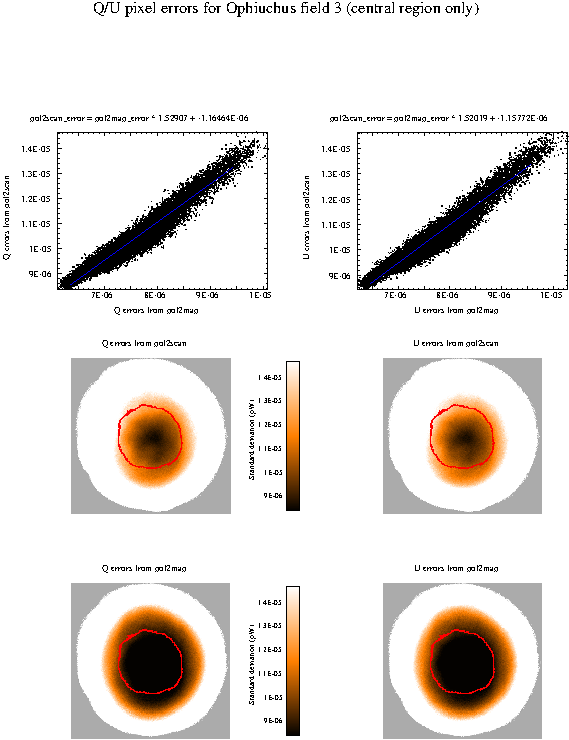
\includepdf[pages={-}]{figs/fig49.pdf}
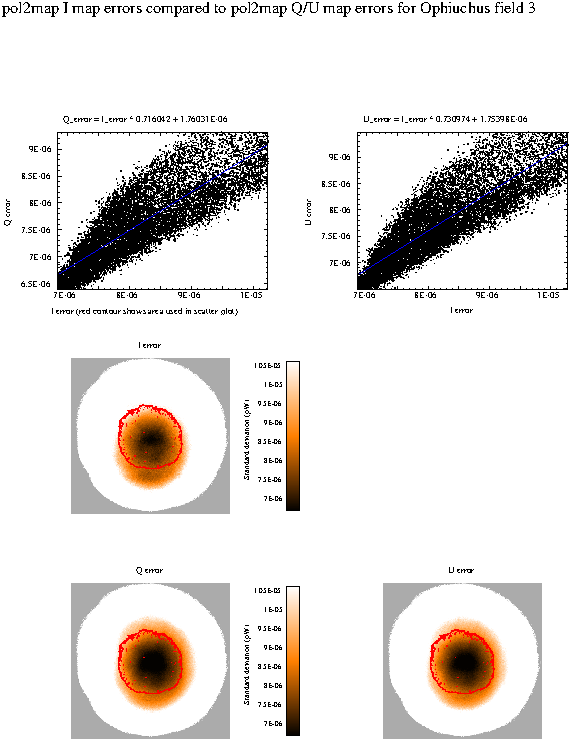
\includepdf[pages={-}]{figs/fig50.pdf}
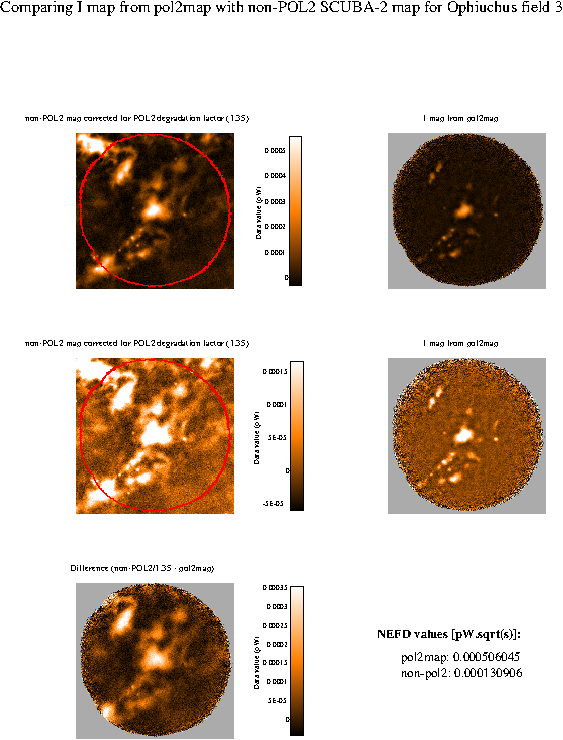
\includepdf[pages={-}]{figs/fig51.pdf}
\includepdf[pages={-}]{figs/fig52.pdf}
\includepdf[pages={-}]{figs/fig53.pdf}
\includepdf[pages={-}]{figs/fig54.pdf}

\subsection{Orion A}
These maps are made from 20 observations of Orion A taken between 20160111
and 20160125.

\includepdf[pages={-}]{figs/fig56.pdf}
\includepdf[pages={-}]{figs/fig57.pdf}
\includepdf[pages={-}]{figs/fig58.pdf}
\includepdf[pages={-}]{figs/fig59.pdf}
\includepdf[pages={-}]{figs/fig60.pdf}
\includepdf[pages={-}]{figs/fig61.pdf}
\includepdf[pages={-}]{figs/fig62.pdf}
\includepdf[pages={-}]{figs/fig63.pdf}

\section{Future work}

\begin{itemize}
\item Further verification of the results presented in section~/ref{sec:results}.
\item \texttt{pol2map} should be used to process some simulated data, so that
we can check that we get out what we put in with sufficient accuracy.
\item As yet no attempt has been made to determine whether these results are
consistent with the canonical value of 1.35 for the POL2 degradation factor at 850
$\mu m$. This could be done by comparing I maps of points sources
created from POL2 observations using \texttt{pol2map}, with maps made
from non-POL2 data using \texttt{makemap} directly. Point sources need to
be used rather than extended sources to avoid complexities caused by the different spatial frequencies
present in POL2 and non-POL2 observations.
\item A more extensive investigation of the NEFD present within POL2 I
maps needs to be performed.
\end{itemize}

\end{document}
